%%%%%%%%%%%%%%%%%%%%%%%%%%%%%%%%%%%%%%%%%
% Uppsala University Assignment Title Page 
% LaTeX Template
% Version 1.0 (27/12/12)
%
% This template has been downloaded from:
% http://www.LaTeXTemplates.com
%
% Original author:
% WikiBooks (http://en.wikibooks.org/wiki/LaTeX/Title_Creation)
% Modified by Elsa Slattegard to fit Uppsala university
% License:
% CC BY-NC-SA 3.0 (http://creativecommons.org/licenses/by-nc-sa/3.0/)

%\title{Title page with logo}
%----------------------------------------------------------------------------------------
%	PACKAGES AND OTHER DOCUMENT CONFIGURATIONS
%----------------------------------------------------------------------------------------

\documentclass[12pt]{article}
\usepackage[english]{babel}
\usepackage[utf8x]{inputenc}
\usepackage{amsmath}
\usepackage{amssymb}
\usepackage{graphicx}
\usepackage{float}
\usepackage{color}
\usepackage[normalem]{ulem}
\usepackage{tabularray}
\usepackage{caption}
\usepackage{subcaption}
\usepackage{cite}
\usepackage{hyperref}
\usepackage[colorinlistoftodos]{todonotes}
\usepackage[ruled,vlined]{algorithm2e}

\setlength {\marginparwidth }{2cm}

\begin{document}
    \begin{titlepage}
    
    \newcommand{\HRule}{\rule{\linewidth}{0.5mm}} % Defines a new command for the horizontal lines, change thickness here
    
    \center % Center everything on the page
     
    %----------------------------------------------------------------------------------------
    %	HEADING SECTIONS
    %----------------------------------------------------------------------------------------
    
    \textsc{\LARGE{T\'{e}cnico Lisboa} \\ \vspace{0.5cm} \LARGE{University of Lisbon}}\\[1cm] % Name of your university/college
    \vspace{-2cm}
    \begin{figure}[H]
        \centering
        \begin{minipage}{.5\textwidth}
            \centering
            \phantom{............}
\includegraphics[width=.9\linewidth]{figures/logos/university-lisbon-logo.png}
        \end{minipage}%
        \begin{minipage}{.5\textwidth}
            \centering
            \hspace{-1cm}
            
\includegraphics[width=.9\linewidth]{figures/logos/tecnico-ulisboa-logo.png}
        \end{minipage}
    \end{figure}
    \vspace{-1cm}
     % Include a department/university logo - this will require the graphicx package
    \textsc{\Large Research Seminar in Information Security}\\[0.5cm] % Major heading such as course name
    \textsc{(Prof. Paulo \uppercase{Mateus})}\\[0.5cm]
    \textsc{Doctoral Program in Information Security}\\[0.5cm] % Minor heading such as course title
    \textsc{\large 2023/2024 - 1\textsuperscript{st} Semester}\\[0.5cm] % Minor heading such as course title
    
    %----------------------------------------------------------------------------------------
    %	TITLE SECTION
    %----------------------------------------------------------------------------------------
    
    \HRule \\[0.3cm]
        { \huge \bfseries Robust Quantum \\ Public-Key Encryption \\ \large (with Applications to Quantum Key Distribution) \\ \vspace{0.5cm} \Large (Giulio \textsc{\uppercase{Malavolta}} - November 23, 2023)}\\[0.4cm] % Title of your document
    \HRule \\[1cm]
     
    %----------------------------------------------------------------------------------------
    %	AUTHOR SECTION
    %----------------------------------------------------------------------------------------
    
    \begin{minipage}{0.75\textwidth}
    
        \begin{flushleft} \large
            \textbf{Report written by:}\\
            \begin{itemize}
                \vspace{-0.1cm}
                \item \normalsize{Rúben \textsc{\uppercase{Barreiro}}:\\
                - \href{mailto:ruben.andre.letra.barreiro@tecnico.ulisboa.pt}{\emph{ruben.andre.letra.barreiro@tecnico.ulisboa.pt}}}
            \end{itemize}
        \end{flushleft}
    
    \end{minipage}\\[2cm]
    \vspace{-1cm}    
    % If you don't want a supervisor, uncomment the two lines below and remove the section above
    %\Large \emph{Author:}\\
    %John \textsc{Smith}\\[3cm] % Your name
    
    %----------------------------------------------------------------------------------------
    %	DATE SECTION
    %----------------------------------------------------------------------------------------
    
    {\large{Last updated: \today}}\\[2cm] % Date, change the \today to a set date if you want to be precise
    
    \vfill % Fill the rest of the page with whitespace

    \end{titlepage}

    \clearpage

    
    \section{Motivation}
    \label{sec:motivation}

    The task of interest in this seminar is to address how to use quantum\break phenomena to build a novel cryptographic protocol for public-key encryption,\break whose security, only relies on the use of authenticated classical channels \cite{malavolta-walter:robust-quantum-public-key-encryption-with-applications-to-quantum-key-distribution:2024:03-2024}.
    
    The Modern Cryptography as we know it today started with the work of Whitfield Diffie and Martin Hellman in 1976, when they showed a Key\break Exchange (KE) protocol, nowadays known as the Diffie-Hellman (DH)\break protocol \cite{merkle:secure-communications-over-insecure-channels:1975:03-2024,diffie-hellman:new-directions-cryptography:1976:03-2024}. This work proposal represents essentially the first time that people performed what we know today as Public Key Encryption (PKE). A couple of years later, namely in 1978, Ron Rivest, Adi Shamir, and Leonard Adleman published together a breakthrough PKE algorithm, today\break known as the Rivest-Shamir-Adleman (RSA) algorithm \cite{rivest-shamir-adleman:method-obtaining-digital-signatures-public-key-cryptosystems:1978:03-2024}, based on the practical difficulty of factoring the product of two large prime numbers. These two research works greatly influenced the Modern Cryptography\break we use nowadays. Indeed, there is a difference between performing a KE\break protocol and a PKE algorithm, in the sense that a KE protocol is an\break interactive protocol and a PKE algorithm is just a two-message protocol, one from a sender party (e.g., Alice) that sends its public key to a receiver (e.g., Bob) and other from the receiver that can use it to encrypt a confidential\break message headed posteriorly to a sender party. Obviously, this KE protocol also works the other way around, where a receiver party can send its public key to a sender, and a sender can use it to encrypt a confidential message headed posteriorly to the receiver party. These work proposals won several prizes, including the Turing Awards, already in the XXI century. We cannot also deny the impact these work proposals had on our lives since it has several\break applications, including social networks (e.g., Facebook and Instagram),\break messaging services (e.g., WhatsApp), Internet and World Wide Web (WWW) and related protocols, such as Hypertext Transfer Protocol Secure (HTTPS) and Transport Layer Security (TLS) protocols, or even global economy, among many other. Actually, there is a famous quote from Silvio Micalli that ends up being true, and that says: ``Cryptographers seldom sleep well''. The reason for that is that essentially, both these two work proposals marked the birth of the Modern Cryptography field as we know it today when they just proposed a cryptographic scheme that allows two parties without previously\break meeting with each other, with the hope that it will be secure forever. In fact,\break each one of these cryptographic schemes comes with the respective security\break assumptions, namely the DH and the RSA assumptions, which work as\break formal proofs that these cryptographic schemes are secure. However, some\break technological and scientific advancements happened in the last years, which led us to want to be sure to have Unconditional Security on the cryptographic schemes we develop today. In simple words, Unconditional Security implies we make no assumptions about the computing power and (technological)\break resources available to an adversary. At this stage, we also know we cannot achieve Unconditional Security for cryptographic tasks such as KE protocols and PKE algorithms unless we bring Quantum Information into the picture.

    \noindent In that direction, we have the famous Bennett-Brassard-1984 (BB84)\break protocol, proposed by Charles Bennett and Gilles Brassard in 1984 \cite{bennett-brassard:quantum-cryptography-public-key-distribution-coin-tossing:1984:03-2024,bennett-brassard:quantum-cryptography-public-key-distribution-coin-tossing:2014:03-2024}, that\break provides the well-desired Unconditional Security once we do not have to trust any Cryptography to have any proven assumption to have security. We can think of the BB84 protocol as a sort of KE protocol similar to the DH\break KE protocol, but we can also use Quantum Cryptography to perform\break the equivalent of the PKE task from the RSA algorithm. However, the BB84 protocol is not considered a standard PKE algorithm, no matter the sort of message we send through it. This quantum cryptographic protocol has at least three rounds of communication between Alice and Bob, for which we can design a ``toy version'' interactive protocol such as illustrated below:

    \vspace{-2ex}
    \begin{figure}[ht]
        \captionsetup{justification=centering}
        \centering
        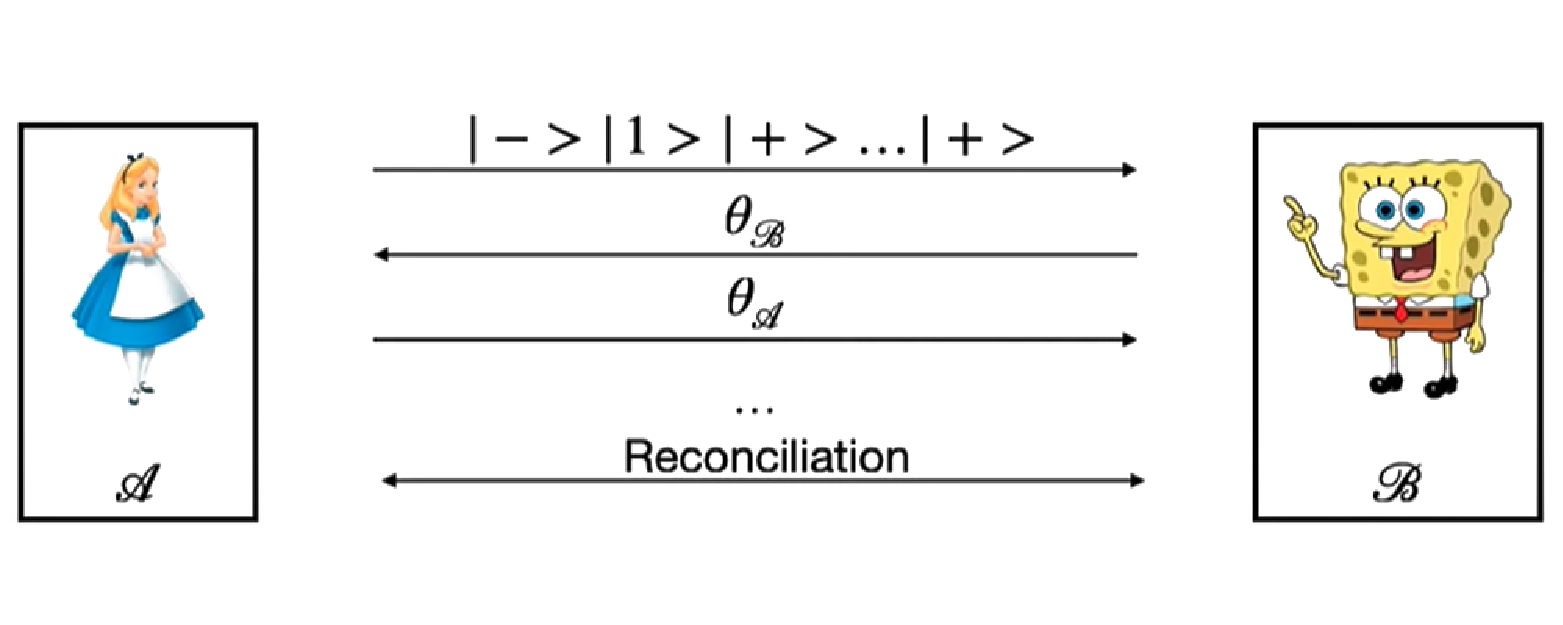
\includegraphics[width=0.8\textwidth]{figures/images/img-1.pdf}
        \caption{High-level illustration of a ``toy version'' of\\ the Bennett-Brassard-1984 (BB84) protocol.}
    \end{figure}
    
    \noindent Namely, the sender starts by sending a bunch of quantum states prepared on some randomly chosen bases to the receiver, for which the receiver measures them on some basis randomly chosen. Then, the receiver sends the bases used for the measurement of those quantum states to the sender, to which the sender replies with the bases used to prepare the quantum states sent. After that, both sender and receiver perform some general error reconciliation steps, and we ultimately know that both parties will agree on a secret key. No matter how we try to simplify this illustrated ``toy version'' protocol, we cannot reduce its round complexity or at least reduce it beyond three rounds.

    However, there is a recent theorem that the author and a colleague proved, saying that if a quantum-secure One-Way Function (OWF) exists, then there exists a two-message round Quantum Key Distribution (QKD) protocol, or in other words, a Quantum Public Key Encryption (QPKE) algorithm with Everlasting Security \cite{malavolta-walter:robust-quantum-public-key-encryption-with-applications-to-quantum-key-distribution:2024:03-2024}. First of all, a two-message round protocol is clearly\break optimal once we know that the sender has to send something and the receiver\break also has to send something. If we choose the standard asynchronous model rather than the simultaneous message model, we conclude we cannot perform\break a KE protocol based on this QKD protocol in less than two message rounds. Second, although we do not achieve Unconditional Security, we achieve\break another form of security known as Everlasting Security. Achieving this form of security is also impossible for both KE protocols and PKE algorithms unless we use quantum information. This fact justifies we are manipulating quantum bits (qubits) instead of just sending (classical) bits in these QKD protocols, such as the BB84 protocol. The concept of Everlasting Security\break essentially says that we can have computational assumptions, but we only have to assume that they hold only during the execution of the protocol.\break Alternatively, the concept of Unconditional Security says that security must also hold after the execution of the protocol and for the whole eternity.\break Practically speaking, Everlasting Security implies we have to assume that a\break (computational) problem must be hard to solve for $30$ seconds, for example,\break and not for $100$ or $1000$ years, which is probably what we usually care about for the security of these PKE algorithms and KE protocols. In some aspects, the Everlasting Security model seems to be a much better computational and security model, reason why we would like to achieve that. Even if we are willing to believe in the security of our protocol against any computational\break assumption, we know that using only classical information jointly with OWFs is insufficient to perform PKE algorithms and KE protocols. Namely, we do not have formal proof for this statement, but we do not have strong evidence\break against it. Another remarkable aspect of this approach is that we only use\break OWFs jointly with these two-message QKD protocols if we manipulate\break quantum information to achieve computational security. Of course, the most substantial part of this protocol is that it is a two-message round protocol if we do not care about rounds of interactions of a usual QKD protocol.

    \noindent Now, we can highlight the differences between Everlasting Security and\break Unconditional Security. For the Everlasting Security model, we admit some\break computational assumptions but only during the execution of the first stage of the protocol. Alternatively, we have no computational assumptions for the Unconditional Security model since the security must last indefinitely,\break independently of technological breakthroughs. We usually also need to use authenticated classical communication channels for the second phase of these quantum cryptographic protocols, which allows us to be sure about who we are talking with during the reconciliation step. However, the existence of an\break authenticated classical communication channel is an extra assumption for the Everlasting Security model, depending on computational assumptions, which\break we only consider during the execution of the unique stage of the protocol.\break This Everlasting Security model is very different from the Unconditional\break Security model from the BB84 protocol, where we have no computational\break

    \definecolor{Gray}{rgb}{0.75,0.75,0.75}
    \begin{table}[htb]
        \captionsetup{justification=centering}
        \centering
        \begin{tblr}{
            width = \linewidth,
            colspec = {Q[456]Q[487]},
            cells = {c},
            cell{1}{1} = {c=2}{0.943\linewidth},
            cell{7}{2} = {fg=Gray},
            cell{8}{2} = {fg=Gray},
            }
            \textbf{Security Model } & \\
            & \\
            \textbf{Everlasting Security} & \textbf{Unconditional Security}\\
            & \\
            {\labelitemi\hspace{\dimexpr\labelsep+0.5\tabcolsep}Needs some\\Computational Assumptions,\\\textit{only during}~the protocol!\\~} & {\labelitemi\hspace{\dimexpr\labelsep+0.5\tabcolsep}Does not need\\Computational Assumptions!}\\
            {\labelitemi\hspace{\dimexpr\labelsep+0.5\tabcolsep}\sout{Use Authenticated\\Classical Channels}} & {\labelitemi\hspace{\dimexpr\labelsep+0.5\tabcolsep}Use Authenticated\\Classical Channels}\\
            & {\hspace*{-0.4\leftmargin}\labelitemii\hspace{\dimexpr\labelsep+0.5\tabcolsep}Needs\\Computational\\Assumptions...}\\
            & {\hspace*{0.7\leftmargin}\labelitemii\hspace{\dimexpr\labelsep+0.5\tabcolsep}... but \textit{only}\\ \phantom{............}\textit{during}\\~ ~ ~ ~ ~ ~ the execution of\\~ ~ ~ ~ ~ ~ ~the protocol!}
        \end{tblr}
        \caption{Overview of the main differences between\\the Everlasting Security and Unconditional Security.}
        \label{tab:overview-main-differences-everlasting-security-and-unconditional-security}
    \end{table}

    \noindent assumptions but still need to authenticate classical information during\break the reconciliation step. Finally, we need an answer to the following question:\break ``How do we get authenticated classical communication channels?''. For that,\break we just need computational assumptions that only have to hold during the\break execution of the protocol. Additionally, the parties must have a pre-shared\break key \textit{a priori} to achieve that authenticated classical communication channel.
    
    \section{Definitions}
    \label{sec:definitions}

    \subsection{Quantum Public Key Encryption (QPKE)}
    \label{subsec:quantum-public-key-encryption}

    First, we need to make clear what means a Quantum Public Key Encryption\break (QPKE) algorithm and define it. In a QPKE algorithm, the sender (i.e., Alice) sends a public key consisting of a classical component denoted as ${pub\_key}_{S}$ through a classical communication channel and a quantum state $\rho$ through a quantum communication channel. Then, the receiver (i.e., Bob) can use this information set to encrypt a message $msg$ using the quantum state $\rho$ and the public key ${pub\_key}_{S}$ that the sender sent. Finally, the sender should be able to recover the message $msg$ back from the encrypted data sent by the receiver. We show an illustrative sketch of this algorithm below:
    
    \begin{figure}[ht]
        \captionsetup{justification=centering}
        \centering
        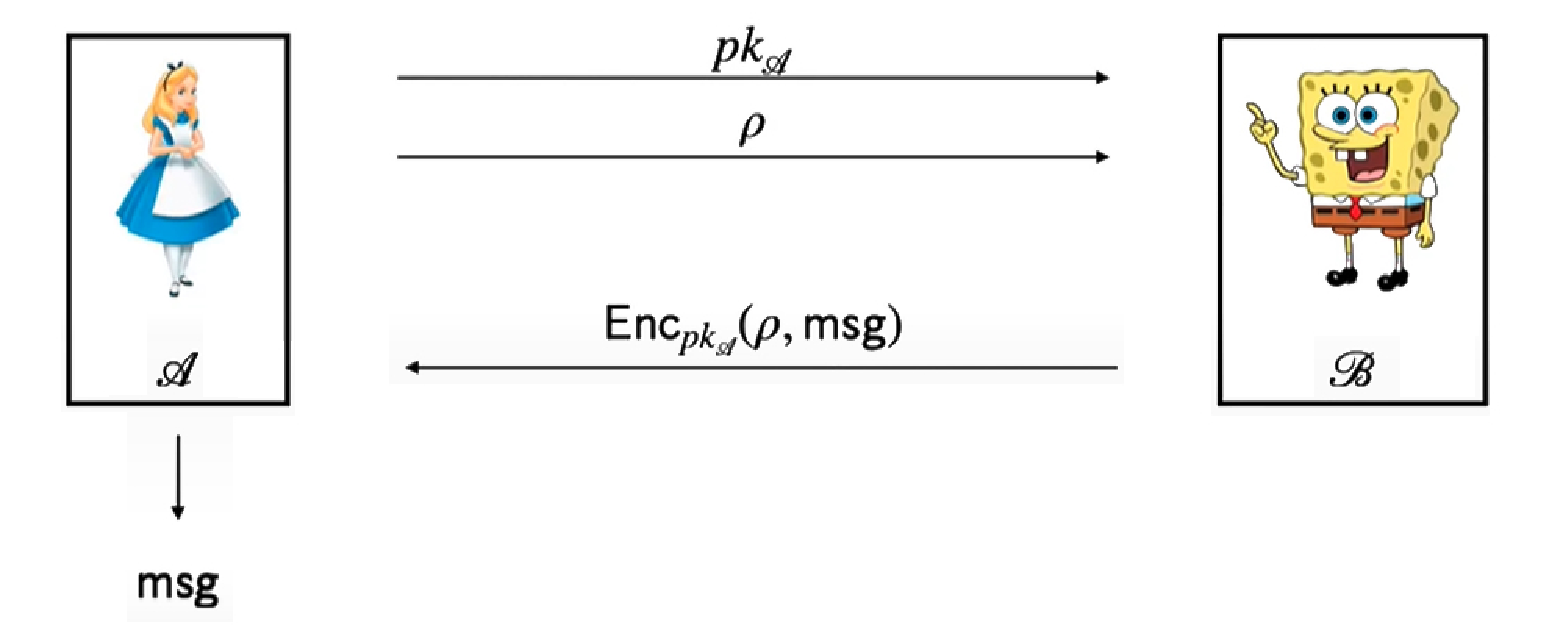
\includegraphics[width=0.8\textwidth]{figures/images/img-2.pdf}
        \caption{High-level illustration of\\ a simple Quantum Public Key Encryption (QPKE) protocol.}
    \end{figure}

    
    
    \noindent Note this particular quantum cryptographic primitive allows the receiver to encrypt any message and offers slightly better functionality than the standard approaches, which suffices for a whole implementation of a QKD protocol.
    
    \subsection{Security Definition}
    \label{subsec:security-definition}

    The security we want is that for all quantum polynomial time adversaries and all pairs of messages $({msg}_{0}, {msg}_{1})$, we are going to define a game where the sender sends the public key ${pub\_key}_{S}$ and the quantum state $\rho$ to an adversary (e.g., Eve). Here, we allow the adversary to perform the operations it wants on this (arbitrary) quantum state $\rho$ once we do not have any authentication on the transmission of the quantum state $\rho$. On the other hand, we assume that the public key ${pub\_key}_{S}$ of the sender is delivered honestly to the receiver in what we can call again an authenticated classical communication channel. On the other hand, we have no assumption on what the quantum state $\rho$ really is. Additionally, even with this strong condition, we want to hide the message $msg$ encrypted by the receiver from the eyes of the adversary. We can think of the quantum state $\rho$ as a quantum component of the output of the public key generation algorithm, along with a classical component, which is a classical secret key extracted from the private key generation algorithm. In this simple experiment, we considered the sample of the quantum state $\rho$ from flipping a coin $c \leftarrow \{0, 1\}$ which results in preparing $|0, {\sigma}_{0}\rangle\langle0,{\sigma}_{0}|$ if $c = 0$ and $|1, {\sigma}_{1}\rangle\langle1,{\sigma}_{1}|$ if $c = 1$, where ${\sigma}_{0}$ and ${\sigma}_{1}$ are two key pairs components generated from the private key ${priv\_key}_{S}$. If we have a perfectly random coin, we end up having the quantum state as a classical mixture given as follows:
    
    $$\rho = \frac{|0, {\sigma}_{0}\rangle\langle0,{\sigma}_{0}| + |1, {\sigma}_{1}\rangle\langle1,{\sigma}_{1}|}{2}$$
    
    \noindent The way we formalize these aspects of the security proof we are defining is to say the adversary can return a quantum state ${\rho}^{*}$ to the receiver, such that the encryption algorithm accepts (i.e., does not abort) with non-negligible\break probability. Therefore, this quantum state ${\rho}^{*}$ would just be delivered to\break the receiver, and the receiver uses it for encrypting the message $msg$.\break Additionally, the trace distance between the quantum state ${\rho}^{*}$ returned when $c = 0$ and the quantum state ${\rho}^{*}$ returned when $c = 1$ both along with\break the adversary's projector $\prod$, should be approximately equal to $0$ and thus negligible in the security parameter $\lambda$ of this (honest) quantum cryptographic protocol. This security claim is given by the mathematical expression below:

    $$ Td({\tau}_{b}) = Td({\tau}_{0}, {\tau}_{1}) = Td \left( \frac{ \prod {\rho}^{*} \prod }{ Tr( \prod {\rho}^{*} ) }, |c,{\sigma}_{c}\rangle\langle c, {\sigma}_{c}| \right) = negl(\lambda) \approx 0 $$
    
    \begin{figure}[ht]
        \captionsetup{justification=centering}
        \centering
        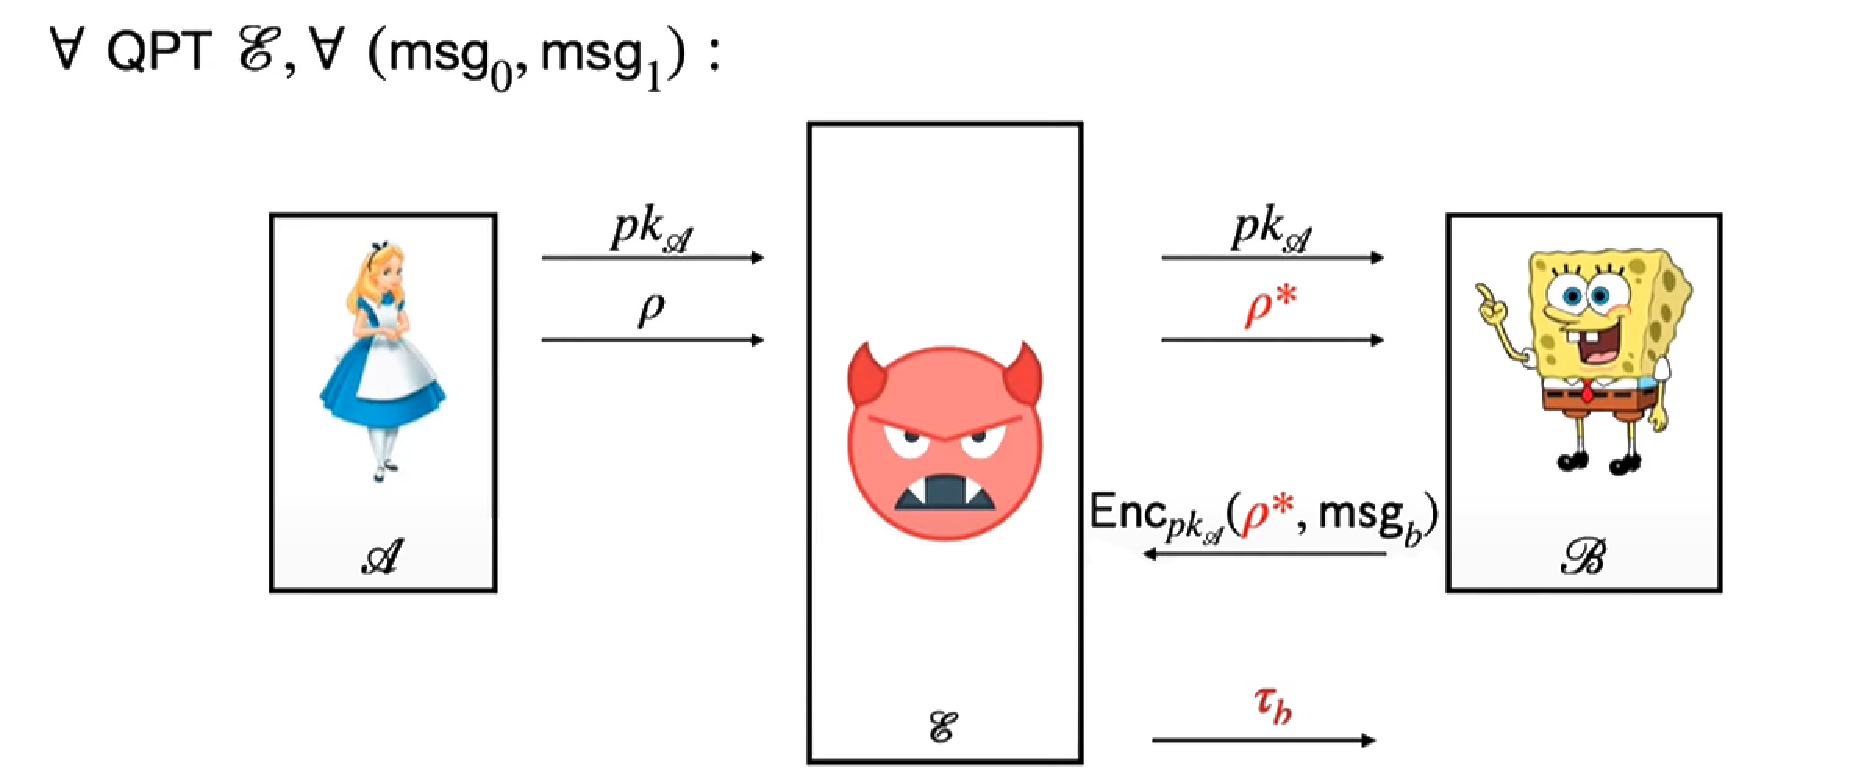
\includegraphics[width=0.8\textwidth]{figures/images/img-3.pdf}
        \caption{High-level illustration of the Security Definition sketch of\\ a simple Quantum Public Key Encryption (QPKE) protocol.}
    \end{figure}

    
    \subsection{One-Time Digital Signatures (OTSs)}
    \label{subsec:one-time-digital-signatures}

    In order to show how this quantum cryptographic protocol works, we need to recall the definition of some required cryptographic primitives. First, we need to recall what is a One-Time Digital Signature or simply One-Time Signature\break (OTS) \cite{lamport:constructing-digital-signatures-from-one-way-function:1979:03-2024}. An OTS is a classical cryptographic primitive consisting of three\break algorithms: a Key Generation, a Signing, and a Verification algorithm. Roughly speaking, this cryptographic primitive allows us to sign a message $msg$, which everyone can verify its authenticity and correctness. There is\break a (very weak) specific security notion called existential unforgeability of\break this cryptographic primitive that demands that nobody else besides the owner of the secret key can sign a message $msg$. Namely, this notion says that an adversary is only allowed to sign a single message of their choice, and even in that case, should not be able to produce a digital signature on\break a new message, or in other words, should be (computationally) hard for\break an adversary to forge a new valid digital signature. Furthermore, another significant point is that OTSs exist if and only if One-Way Functions (OWFs) \cite{diffie-hellman:new-directions-cryptography:1976:03-2024,lamport:constructing-digital-signatures-from-one-way-function:1979:03-2024,goldreich:modern-cryptography-probabilisitic-proofs-pseudorandomness:2013:03-2024} exist. This equivalence claim is a consequence of a research result from the '$70s$, and it is the only cryptographic material we will use here.
    
    
    \subsection{Key Generation (from Sender)}
    \label{subsec:key-generation}

    For the Key Generation algorithm of our quantum cryptographic protocol, we start with the sender party sampling an OTS as a classical component and computing a key pair $(sign\_key, ver\_key)$ for signing and verifying digital\break signatures, respectively. After that, the sender party will also compute the following quantum state $|\psi\rangle$, prepared in a uniform quantum superposition:
    $$ |\psi\rangle = \frac{|0, 0, {\sigma}_{0}\rangle + |1, 1, {\sigma}_{1}\rangle}{\sqrt{2}} $$

    \noindent Here, ${\sigma}_{0}$ is a digital signature on some arbitrary message ${m}_{0}$, and ${\sigma}_{1}$ is\break a digital signature on some arbitrary message ${m}_{1}$. Implicitly, the verification key sampled in this stage of the protocol defines a projective measurement $\left\{ {\prod}_{ver\_key}, I - {\prod}_{ver\_key} \right\}$, which allows anyone to take an arbitrary quantum state and project it onto the span of valid digital signatures composed by the pair of a message and the respective digital signature. Namely, we define the projector ${\prod}_{ver\_key}$ for the verification key $ver\_key$ as presented below:
    $$ {\prod}_{ver\_key} = \sum_{\sigma:\ \mathrm{\text{Verify}}(ver\_key, 0, \sigma) = 1} |0, \sigma\rangle \langle0, \sigma| + \sum_{\sigma:\ \mathrm{\text{Verify}}(ver\_key, 1, \sigma) = 1} |1, \sigma\rangle \langle1, \sigma| $$

    \noindent Note we can efficiently apply this projection operator ${\prod}_{ver\_key}$ if we know the verification key $ver\_key$ once we only need to execute the verification\break algorithm correctly. After that, the sender party will also measure the first register containing the quantum state $|\psi\rangle$ in the Hadamard basis to obtain a single (classical) bit $s \in \{0, 1\}$ that will be a one-time secret key, but first that quantum state $|\psi\rangle$ should be kept in a quantum memory until applying the decryption algorithm on an incoming encrypted message. Thus, the secret key that the sender party ends up obtaining consists of this secret bit $s$ and the residual quantum state $\rho$ sent to the receiver party after measuring the first register containing the quantum state $|\psi\rangle$ in the Hadamard basis.

    
    \subsection{Encryption (from Receiver)}
    \label{subsec:encryption}
    
    For the encryption algorithm, the receiver obtains the residual quantum state $\rho$ from the sender party, checking if that quantum state $\rho$ is in the correct subspace by applying this projection defined by the verification key to that quantum state $\rho$ and see if it succeeds. Otherwise, if the projection fails, the receiver should abort the execution of the protocol. Again, this verification is efficiently implementable, and the essential guarantee we have this operation succeed is that the residual quantum state $\rho$ that consists of a quantum superposition of valid pairs of digital signatures of messages does not have to be strictly equal to the one the sender prepared, but that will be sufficient for us. The receiver proceeds by measuring the projected residual state $\rho$ in the Hadamard basis to obtain a bit string of size $(n + 1)$ we denote as a pair of information $({d}_{1},{d}_{2}) \in \{ 0, 1 \} \times \{{ 0, 1 \}}^{n}$, where ${d}_{1}$ is a single bit, which will work as a One-Time Pad (OTP) key that the receiver uses to mask its message $msg$ and ${d}_{2}$ is a form of auxiliary information for the encryption and decryption algorithms, which will be part of the ciphertext. Therefore, the encrypted message the receiver sends to the sender will be $ct = (msg \oplus {d}_{1}, {d}_{2})$.

    
    \subsection{Decryption (from Sender)}
    \label{subsec:decryption}

    For the decryption algorithm, we first pretend to delay the measurement of the sender party on the first register of the quantum state $|\psi\rangle$ mentioned before on the Hadamard basis, which does not affect the correctness of this quantum cryptographic protocol. Furthermore, we can recall the receiver party also measured the projected quantum state $\rho$ on the Hadamard basis. The rotated quantum state $|\psi\rangle$ in the Hadamard basis has the following form:
    $$ H \times |\psi\rangle = \sum_{d} {(-1)}^{ \left[ d \cdot ( 0, 0, {\sigma}_{0} ) \right] } \times |d\rangle + {(-1)}^{ \left[ d \cdot ( 1, 1, {\sigma}_{1} ) \right] } \times |d\rangle = \sum_{d:\ d \cdot ( 1, 1, {\sigma}_{0} \oplus {\sigma}_{1} ) = 0} |d\rangle $$

    \noindent Namely, this rotated quantum state consists of a quantum superposition of all bit strings $d$ such that this quantum state is orthogonal to them. Therefore, we can verify that this calculation is correct. Then, the measurement of the\break rotated quantum state gives us a bit string $d$ satisfying the following equation:
    $$ d = (s, {d}_{0}, {d}_{1}) \mathrm{\text{, such that }} {d}_{1} \oplus {d}_{2} \cdot ({\sigma}_{0}, {\sigma}_{1}) = s $$
    
    \noindent Note that if we rearrange the equation above, the sender can also compute the term ${d}_{1}$ by performing some rearrangements on the equation above. First, ${d}_{2}$ is part of the ciphertext $ct$ received by the sender. Second, the sender knows ${\sigma}_{0}$ and ${\sigma}_{1}$, as well as the one-time secret key $s$. For that, we must recall the receiver sent the encrypted message $ct = (msg \oplus {d}_{1}, {d}_{2})$, which from computing ${d}_{1}$, the sender can recover the original message $msg$ as well.

    
    \section{Proof Sketch}
    \label{sec:proof-sketch}

    For the proof sketch, we can simplify the proof a little bit but keep its main argument. In the first place, we observe that from the point of view of the attacker who does not see the first measurement from the sender party, the residual quantum state $\rho$ is essentially a classical mixture given as follows:
    
    $$ |0, {\sigma}_{0}\rangle \mathrm{\text{ with probability of }} \frac{1}{2} $$
    
    $$ |1, {\sigma}_{1}\rangle \mathrm{\text{ with probability of }} \frac{1}{2} $$

    \noindent Here, the quantum states $|0, {\sigma}_{0}\rangle$ and $|1, {\sigma}_{1}\rangle$ occur each one with a probability\break of $50\%$ because we traced out the first register of the quantum state $\rho$.
    
    Now, we can recall the first action from the receiver is to project the\break residual quantum state $\rho$ into the span of the pairs of correct digital signatures\break of messages $(b, {\sigma}_{b})$. In other words, the receiver party needs to project the\break residual quantum state $\rho$ onto $\text{Span}( \{ |b, {\sigma}_{b} \rangle: \text{Verify}(ver\_key, b, {\sigma}_{b}) = 1 \} )$.\break The attacker only has two options for passing the projection test and cheating this quantum cryptographic protocol. The attacker must have acted as the identity operator, on what is equivalent to just letting the quantum state pass in the respective quantum communication channel with no action, or it can put some non-trivial amplitude weights on another digital signature. However, this second option is not valid since it breaks unforgeability, which we defined before as a property of our OTS primitives. Namely, for a simple security reduction, given only one digital signature, it is (computationally) hard to compute any non-negligible amplitude weight on the other digital signature. We could measure that quantum state $\rho$ on the Hadamard basis, which results in a quantum superposition of a uniform bit string. Therefore, if we use any bit from the resulting (completely random) uniform bit string $d$ as an OTP primitive, we achieve the well-desired Unconditional Security:
    $$ d \sim \mathrm{\text{Uniform: }} { \{ 0, 1 \} }^{(n + 1)} \longrightarrow \parbox{23ex}{\centering Unconditional Security\\using One-Time Pad}$$

    
    \section{Outlook}
    \label{sec:outlook}

    
    \subsection{Possible Improvements}
    \label{subsec:possible-improvements}

    The author highlights some aspects we can think about possible improvement directions. First, the author and his colleague did not optimize the (initial)\break key rate of this initial work proposal for this quantum cryptographic protocol,\break and they need to improve this feature in the future. Second, the ``na\"{i}ve''\break security model the author and his colleague developed currently only works for noiseless scenarios where we do not need to care about noise nuances, and the protocol should have a better noise tolerance for more realistic\break scenarios. Another aspect the author highlights is that this current quantum\break cryptographic protocol uses large coherent quantum states for the valid pairs of digital signatures of messages, which would imply better quantum\break hardware and larger quantum memories than the currently available ones, turning the implementation of this cryptographic primitive with a reasonable\break security parameter much more difficult at the moment. A possible way to overcome this issue should be to think about a (relatively) equivalent protocol\break with the same round complexity that works qubit-by-qubit, similarly to what happens with most Quantum Key Distribution (QKD) protocols \cite{ekert:quantum-cryptography-based-bell-theorem:1991:03-2024,bennett-brassard-mermin:quantum-cryptography-without-bell-theorem:1992:03-2024,bennett:quantum-cryptography-using-any-two-nonorthogonal-states:1992:03-2024,mu-seberry-zheng:shared-cryptographic-bits-quantized-quadrature-phase-amplitudes-light:1996:03-2024,dagmar:optimal-eavesdropping-quantum-cryptography-six-states:1998:03-2024,bechmann-pasquinucci:incoherent-coherent-eavesdropping-six-state-protocol-quantum-cryptography:1999:03-2024,hwang:quantum-key-distribution-high-loss-toward-global-secure-communication:2003:03-2024,branciard-gisin-kraus-scarani:security-two-quantum-cryptography-protocols-using-same-four-qubit-states:2005:03-2024}, such as the previously mentioned and well-known BB84 protocol \cite{bennett-brassard:quantum-cryptography-public-key-distribution-coin-tossing:1984:03-2024,bennett-brassard:quantum-cryptography-public-key-distribution-coin-tossing:2014:03-2024}. Another\break aspect that the author highlights with a more foundational interest is the\break computational assumptions considered for this quantum cryptographic\break protocol once the author and his colleague considered OWFs sufficient for those assumptions. However, it turns out that we do not believe OWFs to be the minimal assumption in Quantum Cryptography. Namely, if we consider\break quantum states when designing these cryptographic protocols, some\break computational assumptions are believed to be even weaker than OWFs.\break However, the author and his colleague do not know how to achieve the same QPKE protocol from such assumptions because we currently do not have\break concrete candidates other than OWFs for this type of task. Finally, another\break significant point is to verify if this quantum cryptographic protocol can achieve Unconditional Security, and interestingly, we cannot achieve such a property. Actually, there is a very simple counter-example using an attack\break on the model used before for the security definition, even considering an\break authenticated classical communication channel. In this very simple attack, the adversary would essentially keep executing the key generation algorithm until it finds a public key ${pub\_key}_{S}$ that matches the one of the sender party\break and proceeds with the honest cryptographic protocol. For this reason, we cannot expect this protocol to achieve better than Everlasting Security.

    \clearpage

    \begin{figure}[ht]
        \captionsetup{justification=centering}
        \centering
        \vspace{-12ex}
        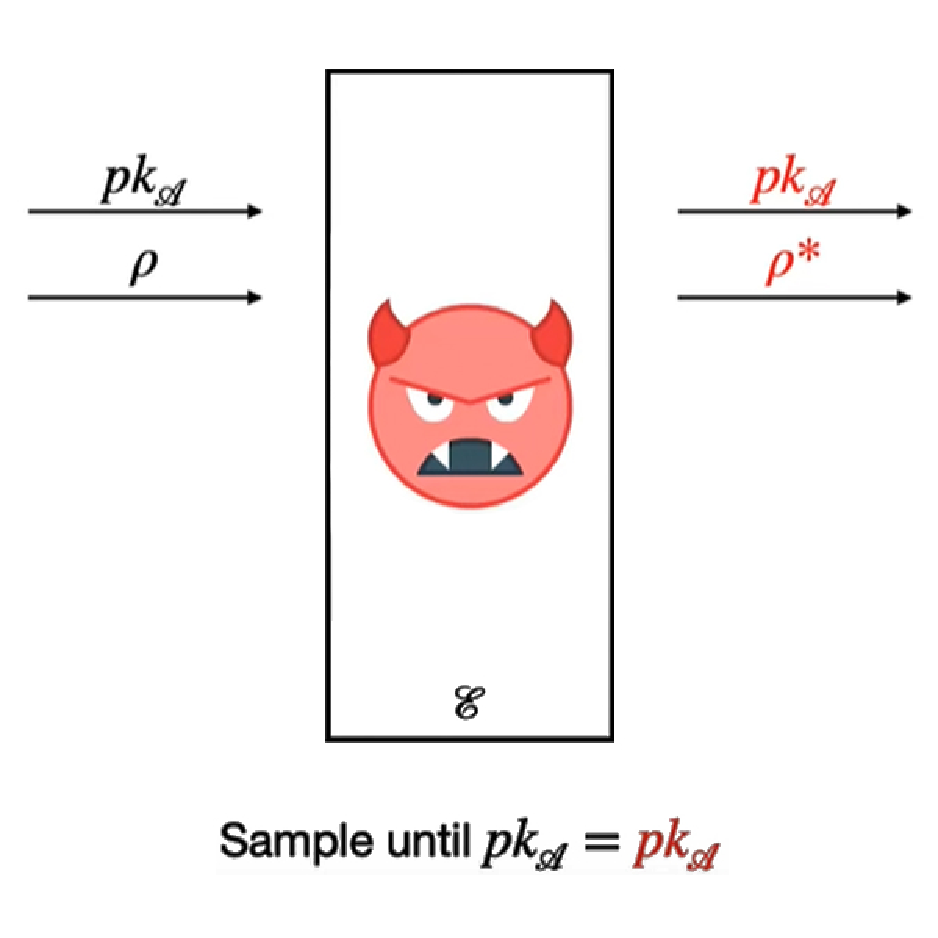
\includegraphics[width=0.5\textwidth]{figures/images/img-4.pdf}
        \caption{High-level illustration of the simple attack used to justify\\ the reason for this Quantum Public Key Encryption (QPKE) protocol not achieving better than Everlasting Security.}
    \end{figure}
    
    
    \subsection{Concurrent Work and Future Work}
    \label{subsec:concurrent-work-and-future-work}

    A concurrent work proposal from Fuyuki Kitagawa, Tomoyuki Morimae,\break Ryo Nishimaki, and Takashi Yamakawa, proposed recently in 2023 \cite{kitagawa-morimae-nishimaki-yamakawa:quantum-public-key-encryption-tamper-resilient-public-keys-one-way-functions:2023:03-2024},\break has extremely similar constructions but results in a slightly different quantum\break cryptographic protocol, where the public keys are quantum, but the\break ciphertexts are classical. The main idea of their work proposal is the same as the one presented in this seminar, but considering only constructions of public encryption from OWFs (or weaker primitives, such as pseudo-random\break function-like states) \cite{ji-liu-song:pseudorandom-quantum-states:2018:03-2024,ananth-qian-yuen:cryptography-pseudorandom-quantum-states:2022-03-2024}. In particular, their cryptographic construction only achieves Computational Security as opposed to the Everlasting Security\break achieved with the QPKE protocol presented in this seminar. However, the quantum cryptographic protocol of this concurrent research work proposal guarantees the secrecy of the encrypted messages even if we assume only unauthenticated quantum communication channels during its execution.

    One possible direction for future work that can be interesting would be to look at other cryptographic primitives beyond PKE algorithms to construct\break new quantum cryptographic protocols similar to the one presented in this seminar and achieve the same level of security as Everlasting Security. Some possible instances of these cryptographic primitives can be quantum variants\break of Identity-Based Encryption (IBE) \cite{shamir:identity-based-cryptosystems-and-signature-schemes:1985:03-2024,cocks:identity-based-encryption-scheme-based-quadratic-residues:2001:03-2024,boneh-franklin:identity-based-encryption-weil-pairing:2003:03-2024}, Attribute-Based Encryption\break (ABE) \cite{shamir:identity-based-cryptosystems-and-signature-schemes:1985:03-2024,sahai-waters:fuzzy-identity-based-encryption:2004:03-2024,goyal-pandey-sahai-waters:attribute-based-encryption-fine-grained-access-control-encrypted-data:2006:03-2024,chase:multi-authority-attribute-based-encryption:2007:03-2024,chase-chow:improving-privacy-security-multi-authority-attribute-based-encryption:2009:03-2024,muller-katzenbeisser-eckert:multi-authority-ciphertext-policy-attributed-based-encryption:2009:03-2024,lewko-waters:decentralizing-attribute-based-encryption:2011:03-2024,jung-li-wan-wan:privacy-preserving-cloud-data-access-multi-authorities:2013:03-2024,jung-li-wan-wan:control-cloud-data-access-privilege-anonymity-fully-anonymous-attribute-based-encryption:2015:03-2024}, as well as Functional Encryption (FE) \cite{sahai-waters:fuzzy-identity-based-encryption:2004:03-2024,boneh-sahai-waters:functional-encryption-definitions-challenges:2011:03-2024,goldwasser-et-al:reusable-garbled-circuits-succinct-functional-encryption:2012:03-2024,gorbunov-vaikuntanathan-wee:attribute-based-encryption-circuits:2013:03-2024,garg-et-al:attribute-based-encryption-circuits-multilinear-maps:2013:03-2024,goldwasser-et-al:how-run-turing-machines-encrypted-data:2013:03-2024}, which are usually built on top of PKE primitives, at least in the classical setting.
    
    
    \bibliographystyle{unsrt}

    \clearpage
    
    \bibliography{bibliography}
    \label{bib:bibliography}
    
\end{document}